
\section*{Problem 4: Neural Network Implementation [51 pts]}
\label{sec:code}

\begin{figure}[H]
    \centering
    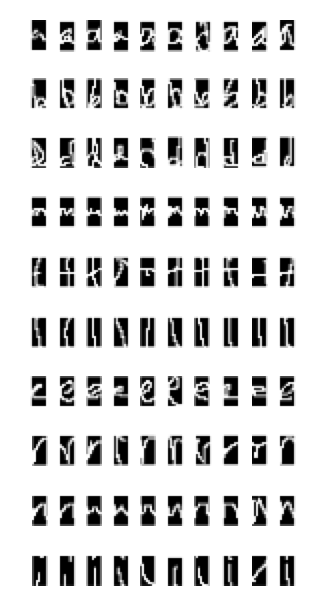
\includegraphics[scale=0.99]{img/10lettergrid.png}
    \caption{10 Random Images of Each of 10 Letters in OCR}
    \label{fig:grid}
\end{figure}

Your goal in this assignment is to label images of handwritten letters by implementing a Neural Network from scratch. You will implement all of the functions needed to initialize, train, evaluate, and make predictions with the network. 

\subsection{The Task and Datasets}
\label{sec:dataset}

\subsubsection*{Datasets} We will be using a subset of an Optical Character Recognition (OCR) dataset. This data includes images of all 26 handwritten letters; our subset will include only the letters ``a," ``e," ``g," ``i," ``l," ``n," ``o," ``r," ``t," and ``u."  The handout contains three datasets drawn from this data: a small dataset with 60 samples per class (50 for training and 10 for \ntset), a medium dataset with 600 samples per class (500 for training and 100 for \ntset), and a large dataset with 1000 samples per class (900 for training and 100 for \ntset). Figure \ref{fig:grid} shows a random sample of 10 images of few letters from the dataset.

\subsubsection*{File Format} Each dataset (small, medium, and large) consists of two csv files---train and \ntset. Each row contains 129 columns separated by commas. The first column contains the label and columns 2 to 129 represent the pixel values of a $16 \times 8$ image in a row major format. Label 0 corresponds to ``a," 1 to ``e," 2 to ``g," 3 to ``i," 4 to ``l," 5 to ``n," 6 to ``o," 7 to ``r," 8 to ``t," and 9 to ``u."
%
Because the original images are black-and-white (not grayscale), the pixel values are either 0 or 1. However, you should write your code to accept arbitrary pixel values in the range [0,1]. The images in Figure \ref{fig:grid} were produced by converting these pixel values into .png files for visualization. Observe that no feature engineering has been done here; instead the neural network you build will \emph{learn} features appropriate for the task of character recognition.


\subsection{Model Definition}

In this assignment, you will implement a single-hidden-layer neural network with a sigmoid activation function for the hidden layer, and a softmax on the output layer. Let the input vectors $\xv$ be of length $M$, the hidden layer $\zv$ consist of $D$ hidden units, and the output layer $\hat{\yv}$ be a probability distribution over $K$ classes. That is, each element $y^k$ of the output vector represents the probability of $\xv$ belonging to the class $k$. 
\\\\\begin{center}
    
\begin{tabular}{ |p{3cm}|p{4cm}|p{3cm}|  }
\hline
\multicolumn{3}{|c|}{Model Architecture} \\
\hline
Input (length) & Layer/Activation & Output (length) \\
\hline
\textbf{x} of length $M$ & Linear (hidden layer) & \textbf{a} of length $D$ \\
\textbf{a} of length $D$ & Sigmoid Activation   & \textbf{z} of length $D$ \\
\textbf{z} of length $D$ & Linear (output layer) & \textbf{b} of length $K$ \\
\textbf{b} of length $K$  & Softmax & \textbf{y} of length $K$ \\
\hline
\end{tabular}
\end{center}\par
\vspace{0.2in}
We can further express this model by adding bias features to the inputs of layers; assume $x^0=1$ is a bias feature on the input and that $z^0=1$ is also fixed. In this way, we have two parameter matrices $\alphav \in \Rb^{D \times (M+1)}$ and $\betav \in \Rb^{K \times (D+1)}$. The extra $0$th column of each matrix (i.e. $\alphav^{\cdot,0}$ and $\betav^{\cdot,0}$) hold the bias parameters. Remember to add the appropriate 0th columns to your inputs/matrices and update the dimensions accordingly (i.e. length $D+1$ instead of $D$). 

\begin{align*}
& a^j = \sum_{m=0}^M \alpha^{jm} x^m \\
& z^j = \frac{1}{1+\exp(-a^j)} \\
& b^k =  \sum_{j=0}^D \beta^{kj} z^j\\
& \hat{y}^k = \frac{\exp(b^k)}{\sum_{l=1}^K \exp(b^l)}\\
\end{align*}
The objective function we're using is the average cross entropy over the training dataset $\Dc = \{ (\xv^{(i)}, \yv^{(i)}) \}$:

\begin{align*}
J(\alphav, \betav)= - \frac{1}{N} \sum_{i=1}^N \sum_{k=1}^{K} y^{(i)^k} \log (\hat{y}^{(i)^k})
\end{align*}

Some points to mention:
\begin{itemize}
\item Do \emph{not} use any machine learning libraries. You may and please do use NumPy.
\item Try to ``vectorize'' your code as much as possible. In Python, you want to avoid for-loops and instead rely on \lstinline{numpy} calls to perform operations such as matrix multiplication, transpose, subtraction, etc. over an entire \lstinline{numpy} array at once. This is much faster; using NumPy over list can speed up your computation by 200x!
\item You'll want to pay close attention to the dimensions that you pass into and return from your functions.
\item Run your implementation locally first against the auto grader, you may need to run it a few times locally to achieve a full score, because of the stochastic nature of the assignment. Once you are able to get a full score locally, submit it to Gradescope. Again note that you may have to submit to Gradescope a few times to get full score, because of the stochastic nature of this assignment.
\end{itemize}
\subsection{Feed Propagation Implementation [8 pts]}
Implement the forward functions for each of the layers: \\ - \texttt{linearForward}, \texttt{sigmoidForward}, \texttt{softmaxForward}, \texttt{crossEntropyForward}. 
\subsubsection{Cross-Entropy $J_{SGD}(\alpha,\beta)$}
Cross-entropy $J_{SGD}(\alpha, \beta)$ for a single example $i$ is defined as follows:
\begin{equation}
\label{eq:celoss2}
J_{SGD}(\alphav, \betav)= - \sum_{k=1}^{K} y^{(i)^k} \log (\hat{y}^{(i)^k})
\end{equation}

$J$ is a function of the model parameters $\alphav$ and $\betav$ because $\hat{y}^{(i)}^k$ is implicitly a function of $\xv^{(i)}$, $\alphav$, and $\betav$ since it is the output of the neural network applied to $\xv^{(i)}$. Of course, $\hat{y}^{(i)^k}$ and $y^{(i)^k}$ are the $k$th components of $\hat{\yv}^{(i)}$ and $\yv^{(i)}$ respectively.
\\\\ The objective function you then use to calculate the average cross entropy over, say the training dataset $\Dc = \{ (\xv^{(i)}, \yv^{(i)}) \}$, is:

\begin{equation}
\label{eq:celoss}
J(\alphav, \betav)= - \frac{1}{N} \sum_{i=1}^N \sum_{k=1}^{K} y^k^{(i)} \log (\hat{y}^{(i)}^k)
\end{equation}
\subsubsection{Complete Forward Pass} 
Next, implement the \texttt{NNForward} function that calls a complete forward pass on the neural network.
\begin{algorithm}[H]
  \caption{Forward Computation}
  \label{alg:forwardmodule}
  \begin{algorithmic}[1] % The number tells where the line numbering should start
    \Procedure{NNForward}{Training example ($\xv$, $\yv$), Parameters $\alphav$, $\betav$}
      \State $\av = \textproc{LinearForward}(\xv, \alphav)$
      \State $\zv = \textproc{SigmoidForward}(\av)$
      \State $\bv = \textproc{LinearForward}(\zv, \betav)$
      \State $\hat{\yv} = \textproc{SoftmaxForward}(\bv)$
      \State $J = \textproc{CrossEntropyForward}(\yv, \hat{\yv})$
      \State \textbf{return} intermediate quantities $\xv,\av,\zv,\bv,\hat{\yv},\Jv$
    \EndProcedure
  \end{algorithmic}
\end{algorithm}
This question will be autograded. You may run the following command locally to run some tests on Q1:
\begin{verbatim}
    python3 autograder.py -q Q1
\end{verbatim}
\vspace{0.3in}
\subsection{Backward Propagation Implementation [12 pts]}
Implement the backward functions for each of the layers: (note: softmax and cross-entropy backpropagation are combined to one due to easier calculation)
\\- \texttt{softmaxBackward}, \texttt{sigmoidBackward}, \texttt{linearBackward}.\\\\
The gradients we need are the matrices of partial derivatives. Let $M$ be the number of input features, $D$ the number of hidden units, and $K$ the number of outputs.

\begin{align}
    &\alphav =
    \begin{bmatrix}
        \alpha^{10} & \alpha^{11} & \dots  & \alpha^{1M} \\
        \alpha^{20} & \alpha^{21} & \dots  & \alpha^{2M} \\
        \vdots      & \vdots      & \ddots & \vdots \\
        \alpha^{D0} & \alpha^{D1} & \dots  & \alpha^{DM}
    \end{bmatrix}
    &&
    \gv_{\alphav} = \frac{\partial J}{\partial \alphav} = 
    \begin{bmatrix}
        \adj{\alpha^{10}} & \adj{\alpha^{11}} & \dots  & \adj{\alpha^{1M}} \\
        \adj{\alpha^{20}} & \adj{\alpha^{21}} & \dots  & \adj{\alpha^{2M}} \\
        \vdots      & \vdots      & \ddots & \vdots \\
        \adj{\alpha^{D0}} & \adj{\alpha^{D1}} & \dots  & \adj{\alpha^{DM}}
    \end{bmatrix}
\end{align}

\begin{align}
    &\betav =
    \begin{bmatrix}
        \beta^{10} & \beta^{11} & \dots  & \beta^{1D} \\
        \beta^{20} & \beta^{21} & \dots  & \beta^{2D} \\
        \vdots      & \vdots      & \ddots & \vdots \\
        \beta^{K0} & \beta^{K1} & \dots  & \beta^{KD}
    \end{bmatrix}
    &&
    \gv_{\betav} = \frac{\partial J}{\partial \betav} = 
    \begin{bmatrix}
        \adj{\beta^{10}} & \adj{\beta^{11}} & \dots  & \adj{\beta^{1D}} \\
        \adj{\beta^{20}} & \adj{\beta^{21}} & \dots  & \adj{\beta^{2D}} \\
        \vdots      & \vdots      & \ddots & \vdots \\
        \adj{\beta^{K0}} & \adj{\beta^{K1}} & \dots  & \adj{\beta^{KD}}
    \end{bmatrix}
\end{align}

Reminder once again that $\alphav$ and $\gv_{\alphav}$ are $D \times (M+1)$ matrices, while $\betav$ and $\gv_{\betav}$ are $K \times (D+1)$ matrices. The $+1$ comes from the extra columns $\alphav^{\cdot, 0}$ and $\betav^{\cdot, 0}$ which are the bias parameters for the first and second layer respectively. We will always assume $x^0 = 1$ and $z^0 = 1$. 
\\\\ Next, implement the \texttt{NNBackward} function that calls a complete backward pass on the neural network.
\begin{algorithm}[H]
  \caption{Backpropagation}
  \label{alg:backpropmodule}
  \begin{algorithmic}[1] % The number tells where the line numbering should start
    \Procedure{NNBackward}{Training example ($\xv$, $\yv$), Parameters $\alphav$, $\betav$, Intermediates $z, \hat{y}$}
      \State Place intermediate quantities $\zv, \hat{\yv}$ in scope
      \State $\gv_{\bv} = \textproc{softmaxBackward*}(\yv, \hat{\yv}$)
      \State $\gv_{\betav}, \gv_{\zv} = \textproc{LinearBackward}(\zv, \betav, \gv_{\bv})$
      \State $\gv_{\av} = \textproc{SigmoidBackward}(\zv, \gv_{\zv})$
      \State $\gv_{\alphav}, \gv_{\xv} = \textproc{LinearBackward}(\xv, \alphav, \gv_{\av})$ \Comment{We discard $\gv_{\xv}$}
      \State \textbf{return} parameter gradients $\gv_{\alphav}, \gv_{\betav}, \gv_{\bv}, \gv_{\zv}, \gv_{\av}$
    \EndProcedure
  \end{algorithmic}
  *It is common to combine the Cross-Entropy and Softmax backpropagation into one, due to the simpler calculation (from cancellation of numerous terms). 
\end{algorithm}
This question will be autograded. You may run the following command to run some tests on Q2:
\begin{verbatim}
    python3 autograder.py -q Q2
\end{verbatim}
\vspace{0.3in}
\subsection{Training with SGD [10 pts]}
\label{sec:sgd}
Implement the \texttt{SGD} function, where you apply stochastic gradient descent to your training. 

For testing on Gradescope, we make a few simplifications: (1) you should \emph{not} shuffle your data and (2) you will use a fixed learning rate. In the real world, you would \emph{not} make these simplifications. 

SGD proceeds as follows, where $E$ is the number of epochs and $\gamma$ is the learning rate.


\begin{algorithm}[H]
  \caption{Stochastic Gradient Descent (SGD) without Shuffle}
  \label{alg:sgd}
  \begin{algorithmic}[1] % The number tells where the line numbering should start
    \Procedure{SGD}{Training data $\Dc$, Validation data $\Dc'$, other relevant parameters} 
      \State Initialize parameters $\alphav, \betav$ \Comment{Use either {\sc Random} or {\sc Zero} from Section \ref{sec:init}}
      \For{$e \in \{1, 2, \ldots, E\}$} \Comment{For each epoch}
        \For{$(\xv, \yv) \in \Dc$} \Comment{For each training example (No shuffling)}
          \State Compute neural network layers:
          %$\hat{\yv} = h_{\alphav, \betav}(\xv)$ and loss $J = \ell(\hat{\yv}, \yv)$ storing intermediate quantities as in 
          \State $\xv, \av, \zv, \bv, \hat{\yv}, J = \textproc{NNForward}(\xv, \yv, \alphav, \betav)$
          \State Compute gradients via backprop: 
            %    $\nabla_{\alphav} J, \nabla_{\betav} J$
          %\State $\gv_{\alphav} = \nabla_{\alphav} J$
          %\State $\gv_{\betav} = \nabla_{\betav} J$ 
          \State 
              $
                \begin{drcases}
                \gv_{\alphav} = \frac{\partial J}{\partial \alphav} \\
                \gv_{\betav} = \frac{\partial J}{\partial \betav}
                \end{drcases} 
                = \textproc{NNBackward}(\xv, \yv, \alphav, \betav, \zv, \hat{y})
              $
          \State Update parameters:
          \State $\alphav \gets \alphav - \gamma \gv_{\alphav}$
          \State $\betav \gets \betav - \gamma \gv_{\betav}$
            %   \State Update parameters:
            %   \State $\alphav \gets \alphav - \gamma \nabla_{\alphav} J$ 
            %   \State $\betav \gets \betav - \gamma \nabla_{\betav} J$ 
        \EndFor
        \State Store training mean cross-entropy $J(\alphav, \betav)$ \Comment{from Eq. \ref{eq:celoss}}
        \State Store validation mean cross-entropy $J(\alphav, \betav)$ \Comment{from Eq. \ref{eq:celoss}}
      \EndFor
      \State \textbf{return} $\alphav, \betav$, cross\_entropy\_train\_list, cross\_entropy\_valid\_list
    \EndProcedure
  \end{algorithmic}
\end{algorithm}

Note that training and validation losses (lines 13, 14) should be calculated \textbf{after} each epoch with the \textbf{updated} $\alpha$ and $\beta$ (which includes running through the training set \textit{again}). 

\subsubsection{Initialization}
\label{sec:init}
In order to use a deep network, we must first initialize the weights and biases in the network. This is typically done with a random initialization, or initializing the weights from some other training procedure. For this assignment, we will be using two possible initialization: 
\begin{quote}
\begin{description}
\item[{\sc Random}] The weights are initialized randomly from a uniform distribution from -0.1 to 0.1. The bias parameters are initialized to zero.
\item[{\sc Zero}] All weights are initialized to 0.  
\end{description}
\end{quote}

You must support both of these initialization schemes.
\vspace{0.15in}

This question is autograded and depends on the correctness to your previous parts. You may run the following command to run some tests on Q3:
\begin{verbatim}
    python3 autograder.py -q Q3
\end{verbatim}
\vspace{0.3in}
\subsection{Label Prediction [5 pts]}
Recall that for a single input $x$, your network outputs a probability distribution over $K$ classes,  $\hat{y}$. After you've trained your network and obtained the weight parameters \textbf{$\alpha$} and \textbf{$\beta$}, you now want to predict the labels given the data.

The error is given by:
\[\mathrm{error} = \frac{\textrm{\# incorrect}}{\textrm{\# total}} = 1 - \textrm{accuracy}\]
\\\\Implement the \texttt{prediction} function as follows.

\begin{algorithm}[H]
  \caption{Prediction}
  \label{alg:predict}
  \begin{algorithmic}[1] % The number tells where the line numbering should start
    \Procedure{prediction}{Training data $\Dc$, Validation data $\Dc'$, Parameters $\alphav, \betav$} 
    \For{$(\xv,\yv) \in \Dc$}
      \State Compute neural network prediction $\hat{\yv}$ from $\textproc{NNForward}(\xv, \yv, \alphav, \betav)$
      \State Predict the label with highest probability $l = \argmax_k \hat{y}^k$
      \State Check for error $l \neq y$
    \EndFor
    \For{$(\xv,\yv) \in \Dc'$}
      \State Compute neural network prediction $\hat{\yv}$ from $\textproc{NNForward}(\xv, \yv, \alphav, \betav)$
      \State Predict the label with highest probability $l = \argmax_k \hat{y}^k$
      \State Check for error $l \neq y$
    \EndFor
    \State \textbf{return} train\_error, valid\_error, train\_predictions, valid\_predictions
    \EndProcedure
  \end{algorithmic}
\end{algorithm}
This question is autograded and depends on the correctness to your previous parts. You may run the following command to run some tests on Q4:
\begin{verbatim}
    python3 autograder.py -q Q4
\end{verbatim}
\vspace{0.3in}
\subsection{Main \texttt{train\_and\_valid} function [4 pts]}
Finally, implement the \texttt{train\_and\_valid()} function to train and validate your neural network implementation. 
\\\\ Your program should learn the parameters of the model on the training data, and report the 1) cross-entropy on both train and validation data for each epoch. After training, it should write out its 2) predictions and 3) error rates on both train and validation data. See the docstring in the code for more details. You may implement any helper code or functions you'd like within \texttt{neural\_network.py}.
%

Your implementation must satisfy the following requirements:
\begin{itemize}
    \item Number of {\bf hidden units} for the hidden layer will be determined by the \texttt{num\_hidden} argument to the \texttt{train\_and\_valid} function.
    \item SGD must support two different {\bf initialization strategies}, as described in Section \ref{sec:init}, selecting between them based on the \texttt{init\_rand} argument to the \texttt{train\_and\_valid} function.
    \item The number of {\bf epochs} for SGD will be determined by the \texttt{num\_epoch} argument to the \texttt{train\_and\_valid} function.
    \item The {\bf learning rate} for SGD is specified by the \texttt{learning\_rate} argument to the \texttt{train\_and\_valid} function.
    \item Perform SGD updates on the training data in the order that the data is given in the input file. Although you would typically shuffle training examples when using stochastic gradient descent, we ask that you {\bf DO NOT} shuffle trials in this assignment.
\end{itemize}
\vspace{0.1in}
This question is autograded and depends on the correctness to your previous parts. You may run the following command to run some tests on Q5:
\begin{verbatim}
    python3 autograder.py -q Q5
\end{verbatim}
\vspace{0.3in}

\subsection{Analysis [12 pts]}
The following questions should be completed after you work through the programming portion of this assignment. The programming portion will be worth 30 points. 

For these questions, \textbf{use the large dataset}. Use the following values for the hyperparameters unless otherwise specified:

\begin{center}
    \begin{tabular}{|c|c|}
        \hline
        \textbf{Parameter} & \textbf{Value} \\
        \hline
        Number of Hidden Units & 50 \\
        \hline
        Weight Initialization & {\sc Random} \\
        \hline
        Learning Rate & 0.01 \\
        \hline
    \end{tabular}
\end{center}


Please submit computer-generated plots for question 1 under sections 2.8.1 and 2.8.2. Include any code required to produce these results in \texttt{additional\_code.py} when submitting the programming component. Note: we expect it to take about \textbf{5 minutes} to train each of these networks.

\subsubsection{Hidden Units [7 pts]}

\begin{enumerate}
    \item \textbf{[5 pts]} Train a single hidden layer neural network using the hyperparameters mentioned in the table above, except for the number of hidden units which should vary among 5, 20, 50, 100, and 200.  Run the optimization for 100 epochs each time.

    Plot the average training cross-entropy (sum of the cross-entropy terms over the training dataset divided by the total number of training examples) on the y-axis vs number of hidden units on the x-axis. In the \textbf{same figure}, plot the average validation cross-entropy.
    
    \begin{tcolorbox}[fit,height=10cm, width=\textwidth, blank, borderline={1pt}{-2pt},nobeforeafter]

    \end{tcolorbox}
    
    \item \textbf{[2 pts]} Examine and comment on the the plots of training and validation cross-entropy. What is the effect of changing the number of hidden units?
    
    \begin{tcolorbox}[fit,height=2cm, width=\textwidth, blank, borderline={1pt}{-2pt},nobeforeafter]

    \end{tcolorbox}
\end{enumerate}

\newpage

\subsubsection{Learning Rate [5 pts]}
\begin{enumerate}
    \item \textbf{[3 pts]} Train a single hidden layer neural network using the hyperparameters mentioned in the table above, except for the learning rate which should vary among 0.1, 0.01, and 0.001. Run the optimization for 100 epochs each time.

    Plot the average training cross-entropy on the y-axis vs the number of epochs on the x-axis for the mentioned learning rates. In the \textbf{same figure}, plot the average validation cross-entropy loss. Make a separate figure for each learning rate.
    
    \begin{tcolorbox}[fit,height=10cm, width=\textwidth, blank, borderline={1pt}{-2pt},nobeforeafter]

    \end{tcolorbox}
    
    \item \textbf{[2 pts]} Examine and comment on the the plots of training and validation cross-entropy. How does adjusting the learning rate affect the convergence of cross-entropy of each dataset?
    
    \begin{tcolorbox}[fit,height=2cm, width=\textwidth, blank, borderline={1pt}{-2pt},nobeforeafter]

    \end{tcolorbox}
\end{enumerate}

\subsection{Submission}

Upload \texttt{neural\_network.py} and \texttt{additional\_code.py} to Gradescope. Your submission should finish running within 20 minutes, after which it will time out on Gradescope.

Don't forget to include any request results in the PDF of the Written component, which is to be submitted on Gradescope as well.

You may submit to Gradescope as many times as you like. You may also run the autograder on your own machine to speed up the development process. Just note that the autograder on Gradescope will be slightly different than the local autograder. The autograder can be invoked on your own machine using the command:

\begin{verbatim}
python3.6 autograder.py
\end{verbatim}

Note that running the autograder locally will not register your grades with us. Remember to submit your code when you want to register your grades for this assignment.

The autograder on Gradescope might take a while but don't worry; so long as you submit before the deadline, it's not late.






